\documentclass[11pt]{article}
\usepackage[a4paper,margin=1in]{geometry}
\usepackage{amsmath,amssymb,amsfonts}
\usepackage{booktabs}
\usepackage{graphicx}
\usepackage{caption}
\usepackage{enumitem}
\usepackage[hidelinks]{hyperref}
\usepackage{xurl}
\usepackage{microtype}
\usepackage{array}
\usepackage[table]{xcolor}

\title{A Mechanism Report on Symmetric Membrane Continuation and Exit Timing in the 2D One-Target Model}
\author{}
\date{}

\setlist{nosep}
\setlength{\textfloatsep}{8pt plus 2pt minus 2pt}
\setlength{\floatsep}{6pt plus 2pt minus 2pt}
\setlength{\intextsep}{6pt plus 2pt minus 2pt}
\setlength{\abovecaptionskip}{4pt}
\setlength{\belowcaptionskip}{0pt}
\setlength{\tabcolsep}{5pt}
\renewcommand{\arraystretch}{1.10}

\begin{document}
\maketitle

\section*{Executive Summary}
This companion report isolates one specific question for the symmetric one-target membrane baseline: \emph{when do trajectories first leave the corridor, and when do they genuinely cross the membrane?}

The main conclusions are:
\begin{enumerate}
  \item The double-peak structure is already present in the fully reflective control. Under the symmetric permeability continuation from \(\kappa=0\) to \(\kappa=0.006\), the system stays in \texttt{phase=1}; the membrane does not create the bimodality from scratch.
  \item In the fully reflective case, \(\tau_{\mathrm{mem}}\) is identically absent, but \(\tau_{\mathrm{out}}\) can still be nonzero because the left opening allows outside detours.
  \item The later windows are mainly associated with trajectories that leave the main corridor early and only return much later, rather than trajectories that get stuck near the target funnel.
  \item Membrane crossings do enhance the later windows; if \(\kappa\) is pushed into a critical band, the membrane-assisted mass in \texttt{peak2} eventually exceeds \(50\%\) around \(\kappa\approx 0.014\). However, this takeover occurs only right before collapse: \texttt{phase=1} survives only up to \(\kappa=0.0152\), and by \(\kappa=0.0153\) the system has already fallen to \texttt{phase=0}.
\end{enumerate}

\section{Baseline and Timing Observables}
The report fixes the symmetric one-target corridor-only soft-bias baseline
\[
L_x=60,\qquad W_y=15,\qquad (x_s,y_s)=(7,7),\qquad (x_t,y_t)=(58,7),
\]
with corridor band \(y=5,\dots,9\) and membrane span \(x=5,\dots,54\). The local rightward bias acts only on the main corridor segment \(5\le x\le 54,\ 5\le y\le 9\), with
\[
\delta_{\mathrm{core}}=0.8,\qquad \delta_{\mathrm{open}}=0.0,
\]
while the whole domain still carries a weak global leftward drift \((b_x,0)=(-0.08,0)\). We then scan the symmetric membrane permeability
\[
\kappa_{c\to o}=\kappa_{o\to c}=\kappa\in\{0,0.00025,\dots,0.0060\},
\]
and recompute the exact \(f(t)\), the three bimodality windows, and both timing observables at each \(\kappa\) using the common long horizon \(t_{\max}=40000\).
To answer whether the membrane-assisted family can ever take over the late peak, the report also includes a dedicated critical-band probe over
\[
\kappa\in\{0.0120,0.0130,0.0140,0.0145,0.0148,0.0149,0.0150,0.0151,0.0152,0.0153\}.
\]

The two first-event times are
\[
\tau_{\mathrm{out}}=\inf\{t\ge 1: X_t\notin C\},
\qquad
\tau_{\mathrm{mem}}=\inf\{t\ge 1:(X_{t-1},X_t)\in E_{\mathrm{mem}}^{c\to o}\},
\]
where \(C\) is the corridor band and \(E_{\mathrm{mem}}^{c\to o}\) is the set of directed corridor-to-outside membrane edges. The distinction is essential:
\begin{itemize}
  \item \(\tau_{\mathrm{out}}\) records the first time the path leaves the corridor, no matter whether this happens through the left opening or through a membrane crossing;
  \item \(\tau_{\mathrm{mem}}\) records only genuine membrane crossings.
\end{itemize}
Therefore \(\tau_{\mathrm{out}}\) can be nonzero even at \(\kappa=0\), while \(\tau_{\mathrm{mem}}\) must vanish there.

The three windows are still determined by the repo-native rule: for each \(\kappa\), the smoothed \(f(t)\) supplies \(t_{\mathrm{peak1}}, t_{\mathrm{valley}}, t_{\mathrm{peak2}}\), and a common half-width. To align the representative panels with the mechanism thresholds, the remainder of the report uses
\[
\kappa=0,\qquad \kappa=0.0140\ \text{(takeover onset)},\qquad \kappa=0.0152\ \text{(last phase-1)}.
\]
At these three values the late peak locations are \(2359, 2028, 1968\), while \(\mathrm{sep}_{\mathrm{peaks}}\) decreases from \(0.447\) to \(0.289\) and then \(0.273\).

\begin{figure}[!htbp]
  \centering
  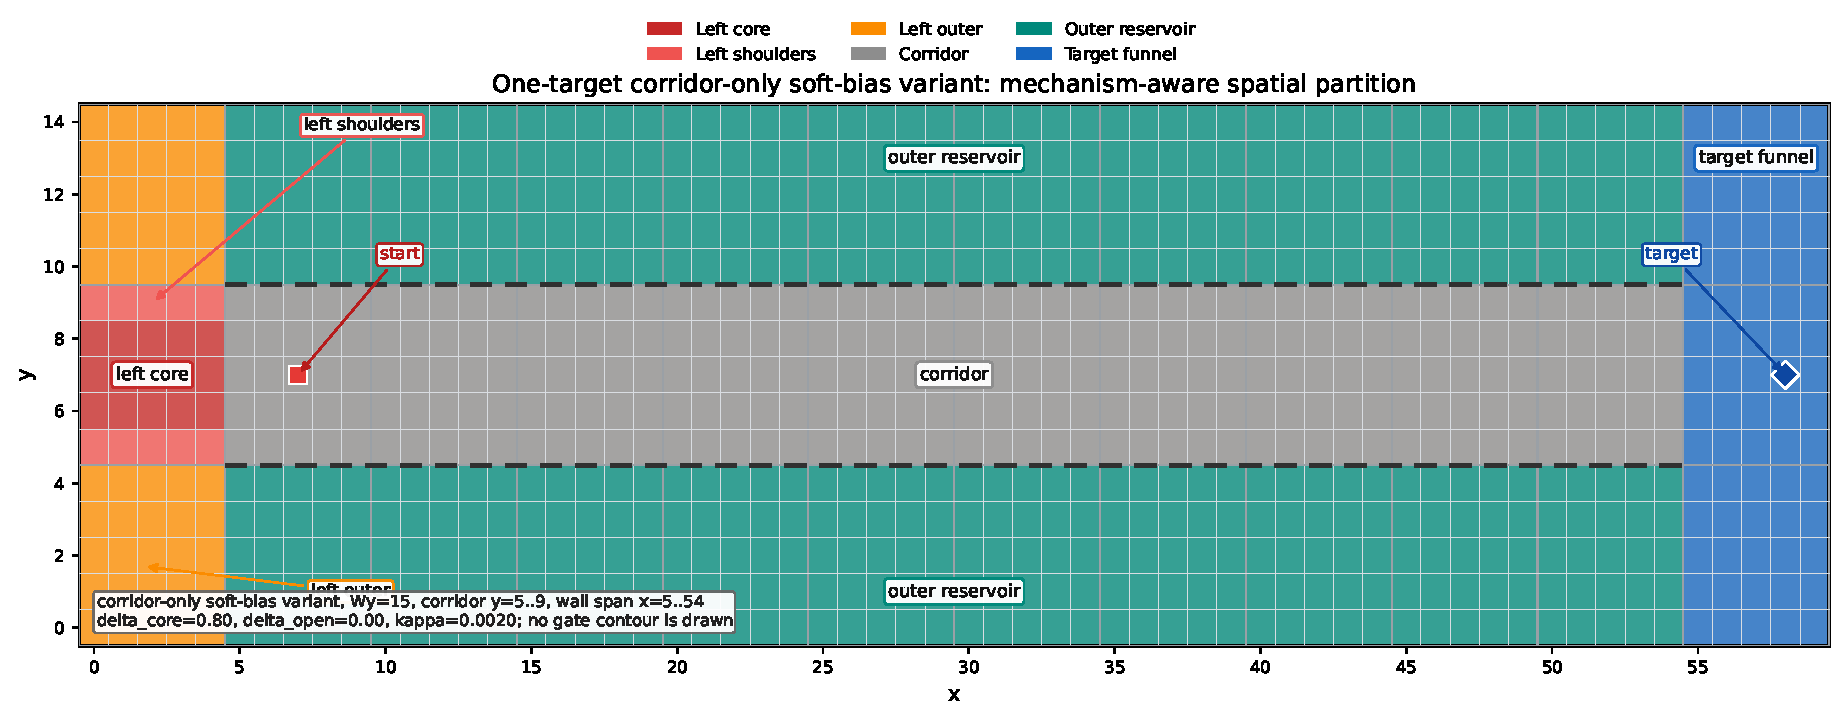
\includegraphics[width=0.82\linewidth]{../artifacts/figures/one_target_partition.pdf}
  \caption{Spatial partition reused from the symmetric one-target explainer report. For the present report, the key distinction is between the left-side regions, the corridor band, and the outside states. Leaving the corridor means entering the outside states for the first time.}
  \label{fig:partition}
\end{figure}

\section{Symmetric Membrane Continuation}
\begin{figure}[!htbp]
  \centering
  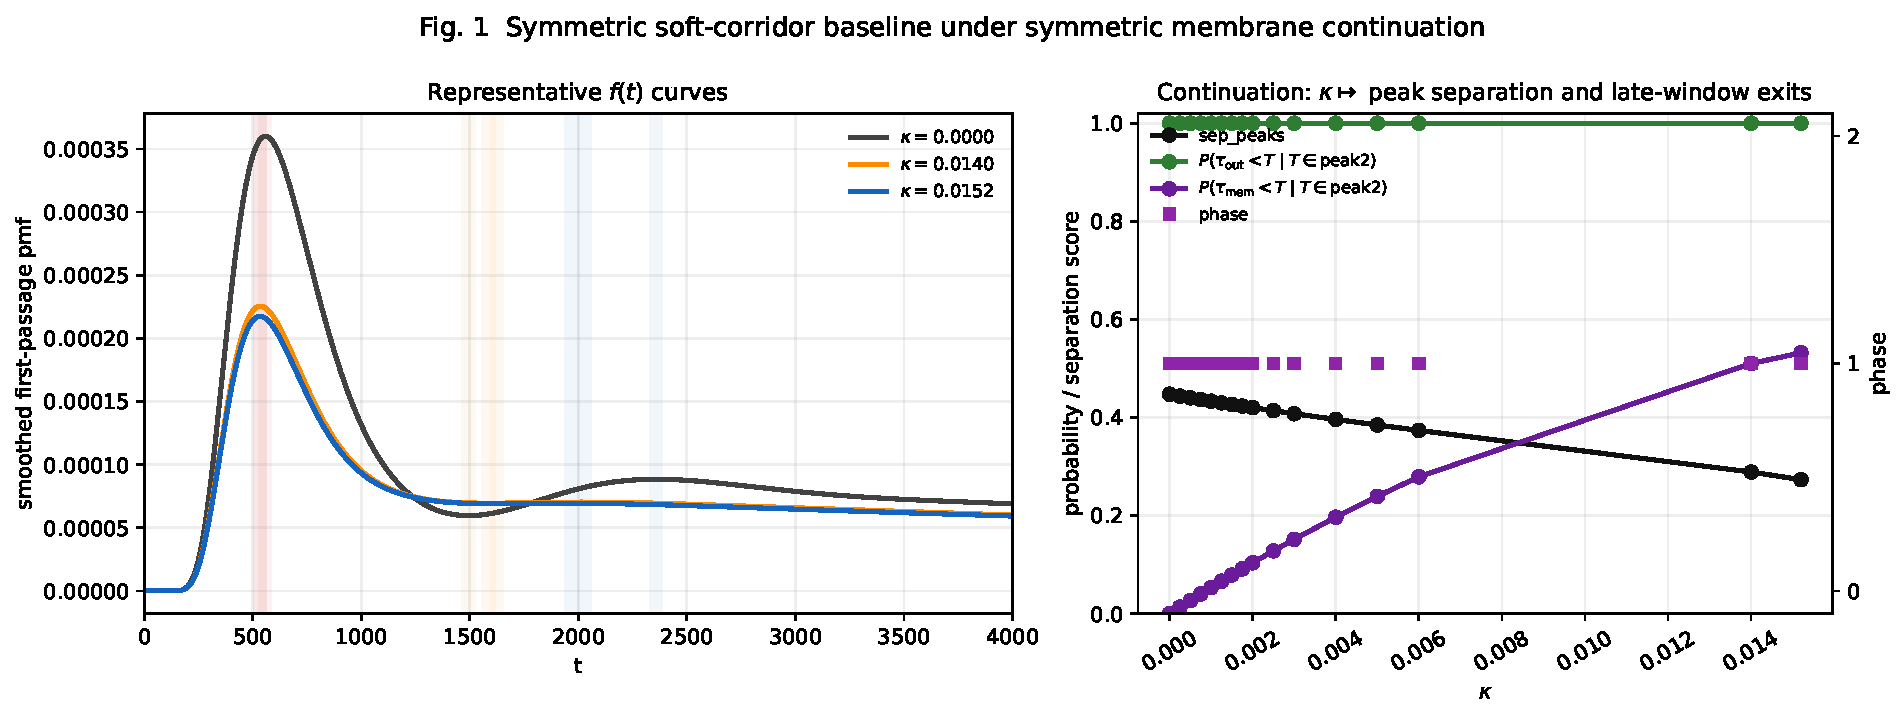
\includegraphics[width=0.98\linewidth]{../artifacts/figures/fig1_kappa_continuation.pdf}
  \caption{Symmetric permeability continuation. Left: representative smoothed \(f(t)\) curves for \(\kappa=0\), takeover onset \(\kappa=0.0140\), and the last phase-1 case \(\kappa=0.0152\). Right: scan summary showing \(\mathrm{sep}_{\mathrm{peaks}}(\kappa)\), phase\((\kappa)\), \(P(\tau_{\mathrm{out}}<T\mid T\in\texttt{peak2})\), and \(P(\tau_{\mathrm{mem}}<T\mid T\in\texttt{peak2})\).}
  \label{fig:kappa-cont}
\end{figure}

Figure~\ref{fig:kappa-cont} makes three points clear.

First, the soft-corridor baseline remains bimodal but never becomes a clear double peak along this continuation: the system stays in \texttt{phase=1} throughout.

Second, \(\mathrm{sep}_{\mathrm{peaks}}\) decreases steadily as \(\kappa\) increases. In this parameter regime, the membrane does not generate the double peak; if anything, it compresses the peak separation, from about \(0.447\) at baseline to about \(0.273\) at the last phase-1 point.

Third, \(P(\tau_{\mathrm{out}}<T\mid T\in\texttt{peak2})\) is already essentially \(1\), while \(P(\tau_{\mathrm{mem}}<T\mid T\in\texttt{peak2})\) rises from \(0\) to about \(51.0\%\) at takeover onset and \(53.2\%\) at the last phase-1 point. So the membrane-assisted subfamily does eventually become the majority within the late peak, but only in the narrow pre-collapse band rather than across a broad stable bimodal regime.

\section{Takeover Occurs Only Right Before Collapse}
\begin{figure}[!htbp]
  \centering
  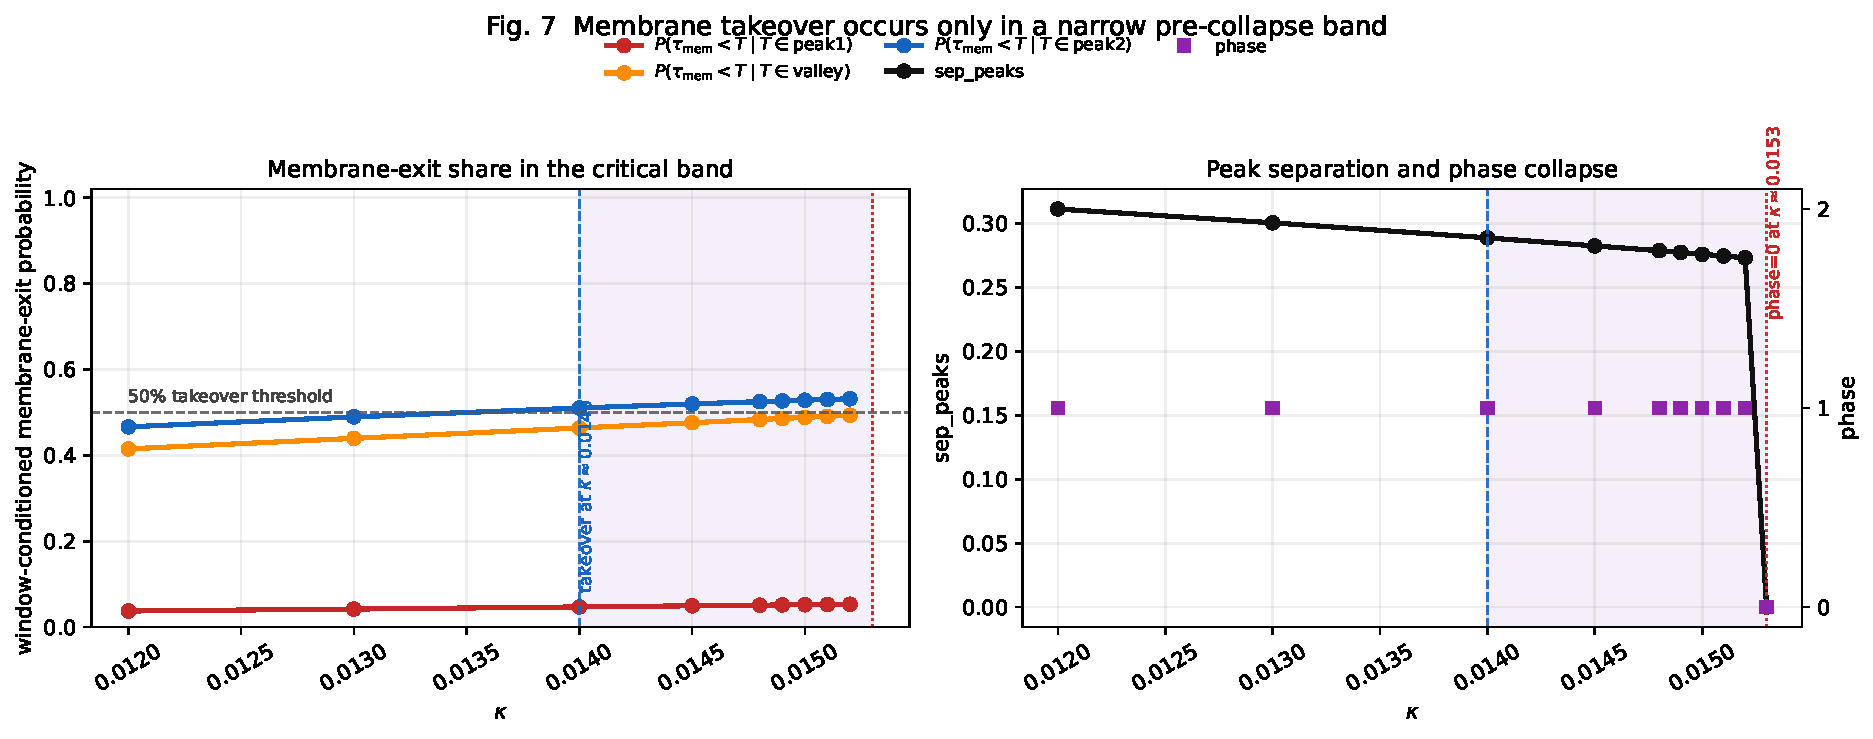
\includegraphics[width=0.98\linewidth]{../artifacts/figures/fig7_takeover_before_collapse.pdf}
  \caption{Critical-band probe. Left: membrane-exit probabilities in \texttt{peak1}, \texttt{valley}, and \texttt{peak2}; the dashed \(50\%\) line marks the point where the membrane-assisted mass becomes the majority. Right: \(\mathrm{sep}_{\mathrm{peaks}}\) and phase in the same band, showing how little room remains between takeover and collapse.}
  \label{fig:takeover}
\end{figure}

Figure~\ref{fig:takeover} sharpens the continuation picture.

First, the membrane-assisted late family does keep growing, and for the late peak it first exceeds \(50\%\) at approximately
\[
\kappa\approx 0.0140.
\]
At that point,
\[
P(\tau_{\mathrm{mem}}<T\mid T\in\texttt{peak2})\approx 51.0\%,
\]
so membrane-assisted trajectories are no longer a small correction inside the late peak.

Second, this does \emph{not} create a broad, stable membrane-dominated bimodal regime. Instead, \texttt{phase=1} survives only up to
\[
\kappa=0.0152,
\]
while by
\[
\kappa=0.0153
\]
the system has already dropped to \texttt{phase=0}. Over the same narrow band, \(\mathrm{sep}_{\mathrm{peaks}}\) decreases further from about \(0.311\) to about \(0.273\).

Third, the mechanism picture is therefore:
\begin{quote}
membrane-assisted paths can take over the second peak while bimodality is still detectable, but only in a very narrow pre-collapse window rather than in a broad membrane-dominated phase.
\end{quote}

This strengthens the earlier conclusion: in the weak-to-moderate permeability regime, the second peak is still governed primarily by outside detours and rollback. The membrane-assisted branch becomes the majority only when the peak separation is already on the verge of collapsing.

\section{What the Critical Point Looks Like in the Curves}
\begin{figure}[!htbp]
  \centering
  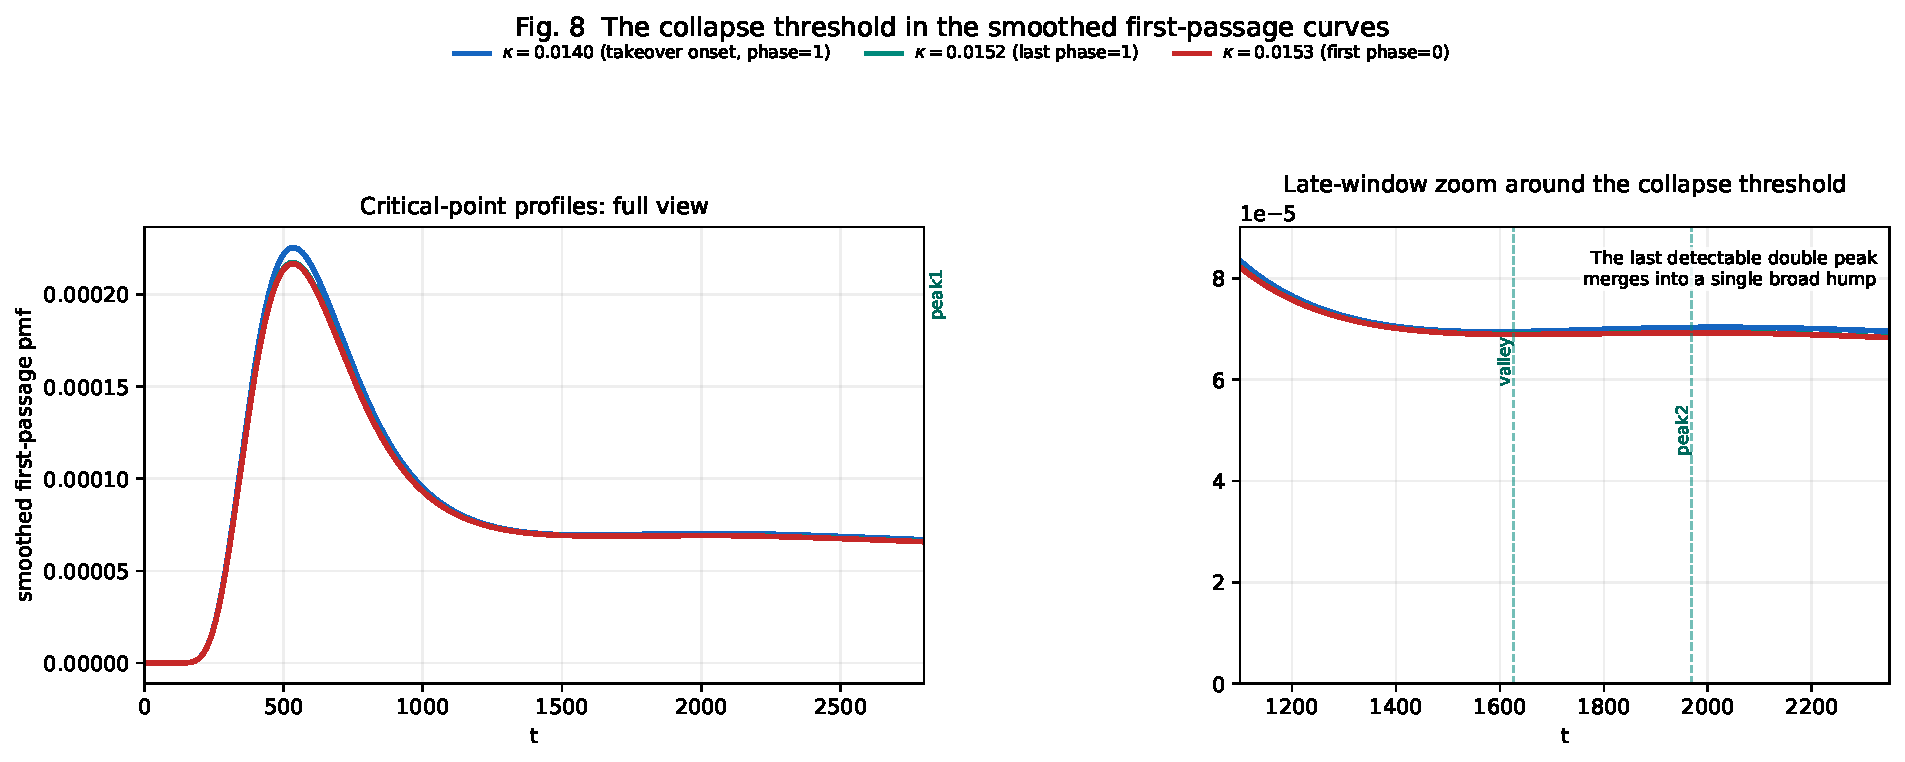
\includegraphics[width=0.98\linewidth]{../artifacts/figures/fig8_critical_collapse_curves.pdf}
  \caption{Smoothed \(f(t)\) profiles near the collapse threshold. The three curves correspond to \(\kappa=0.0140\) (takeover onset), \(\kappa=0.0152\) (the last \texttt{phase=1} case), and \(\kappa=0.0153\) (the first \texttt{phase=0} case). The right panel zooms into the late-peak region so the merger of the second peak into a broad single hump can be seen directly.}
  \label{fig:critical-curves}
\end{figure}

If the goal is simply to \emph{see} the critical threshold, Figure~\ref{fig:critical-curves} is the clearest picture.

The left panel shows that from \(\kappa=0.0140\) to \(\kappa=0.0152\), the overall first-passage profile still retains a detectable two-timescale structure. By \(\kappa=0.0153\), however, the same repo-native criterion no longer classifies the profile as bimodal.

The right panel is the key close-up. In the late-time region:
\begin{itemize}
  \item at \(\kappa=0.0152\), one can still distinguish a second broad rise after the early peak;
  \item at \(\kappa=0.0153\), that second rise has merged back into a flatter, wider single hump/shoulder.
\end{itemize}

So the present ``critical point'' should be read as a practical mechanism threshold rather than an infinitely sharp mathematical phase transition:
\begin{quote}
at \(\kappa=0.0152\), the profile is still usefully described as bimodal; by \(\kappa=0.0153\), it has already collapsed into a single-hump shape under the same detection rule.
\end{quote}

\section{Fully Reflective Control}
\begin{figure}[!htbp]
  \centering
  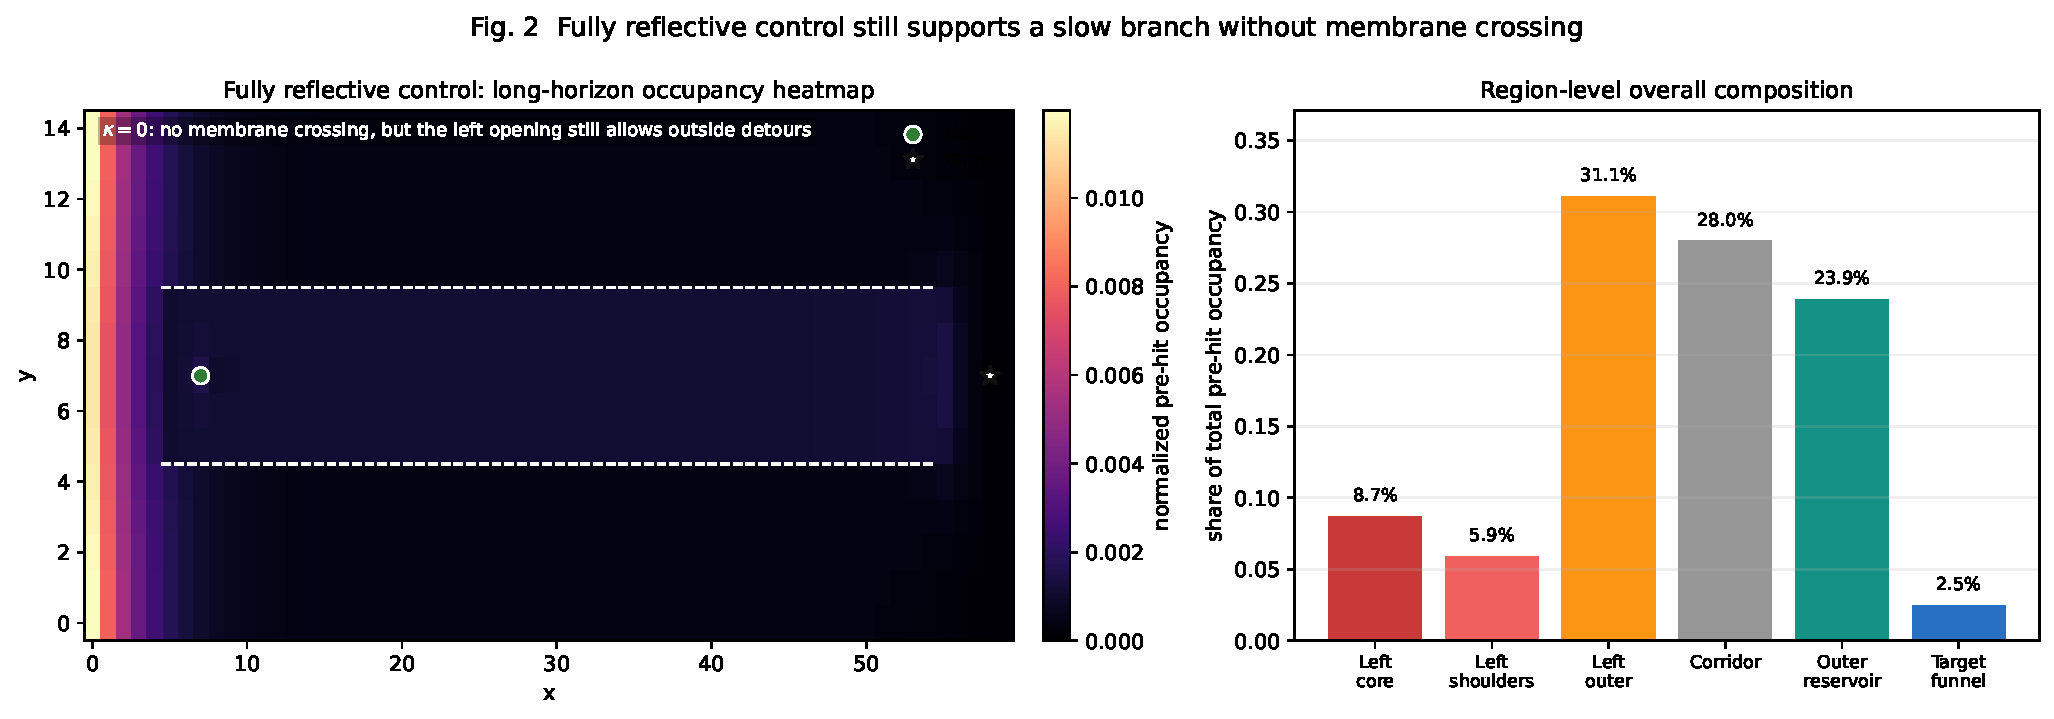
\includegraphics[width=0.98\linewidth]{../artifacts/figures/fig2_fully_reflective_overall_distribution.pdf}
  \caption{Overall pre-hit occupancy for the fully reflective control \((\kappa=0)\). Left: long-horizon occupancy heatmap. Right: total occupancy mass aggregated over the six mechanism regions.}
  \label{fig:fully-refl}
\end{figure}

Figure~\ref{fig:fully-refl} provides the key zero-membrane control. In this case:
\begin{itemize}
  \item \(\tau_{\mathrm{mem}}\) is impossible;
  \item yet `left outer`, `corridor`, and `outer reservoir` still carry most of the total pre-hit occupancy.
\end{itemize}
Numerically, the long-horizon occupancy is approximately
\[
\texttt{left outer}=31.1\%,\quad
\texttt{corridor}=28.0\%,\quad
\texttt{outer reservoir}=23.9\%.
\]
This already demonstrates that a slow branch exists even at \(\kappa=0\): it is created by outside detours through the left opening rather than by membrane crossings.

\section{\texorpdfstring{\(\tau_{\mathrm{out}}\)}{tau_out}: When Is the Corridor Left for the First Time?}
\begin{figure}[!htbp]
  \centering
  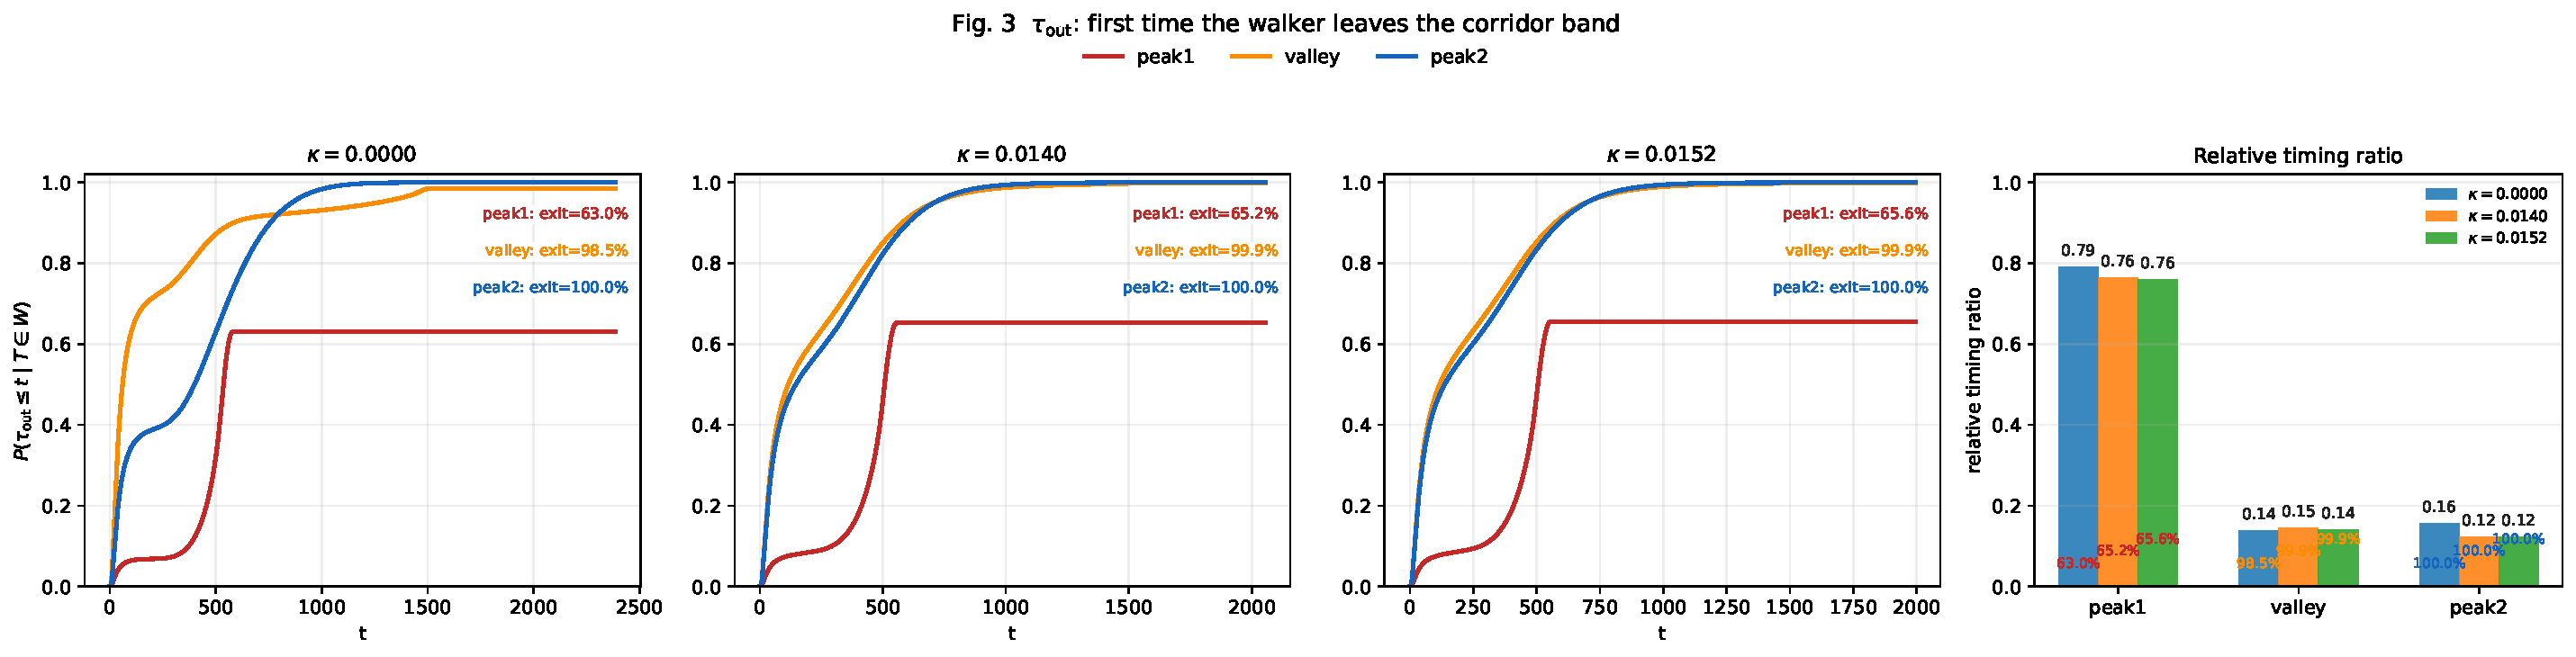
\includegraphics[width=0.98\linewidth]{../artifacts/figures/fig3_tau_out_timing.pdf}
  \caption{Window-conditioned CDFs and relative timing ratios for \(\tau_{\mathrm{out}}\). The three CDF panels correspond to \(\kappa=0\), \(\kappa=0.0140\), and \(\kappa=0.0152\); the right panel reports
  \(
  E[\tau_{\mathrm{out}}\mid \tau_{\mathrm{out}}<T,\ T\in W]/E[T\mid T\in W].
  \)}
  \label{fig:tau-out}
\end{figure}

Figure~\ref{fig:tau-out} tells us when the path first leaves the corridor band.

Three features stand out:
\begin{itemize}
  \item only about \(63\%\) of the \texttt{peak1} trajectories leave the corridor before hitting the target;
  \item almost all \texttt{valley} and \texttt{peak2} trajectories do so, with probabilities around \(98.5\%\) and \(100\%\);
  \item even at takeover onset and at the last phase-1 point, these later-window corridor exits still happen very early relative to the final hitting time, with timing ratios only around \(0.12\) to \(0.15\).
\end{itemize}

This supports a clean interpretation of the late branch: those trajectories do not wait until the very end to leave the corridor. They typically peel away from the corridor early, spend a long time on a detour, and only later return to finish the hit.

\section{\texorpdfstring{\(\tau_{\mathrm{mem}}\)}{tau_mem}: When Does the First Genuine Membrane Crossing Occur?}
\begin{figure}[!htbp]
  \centering
  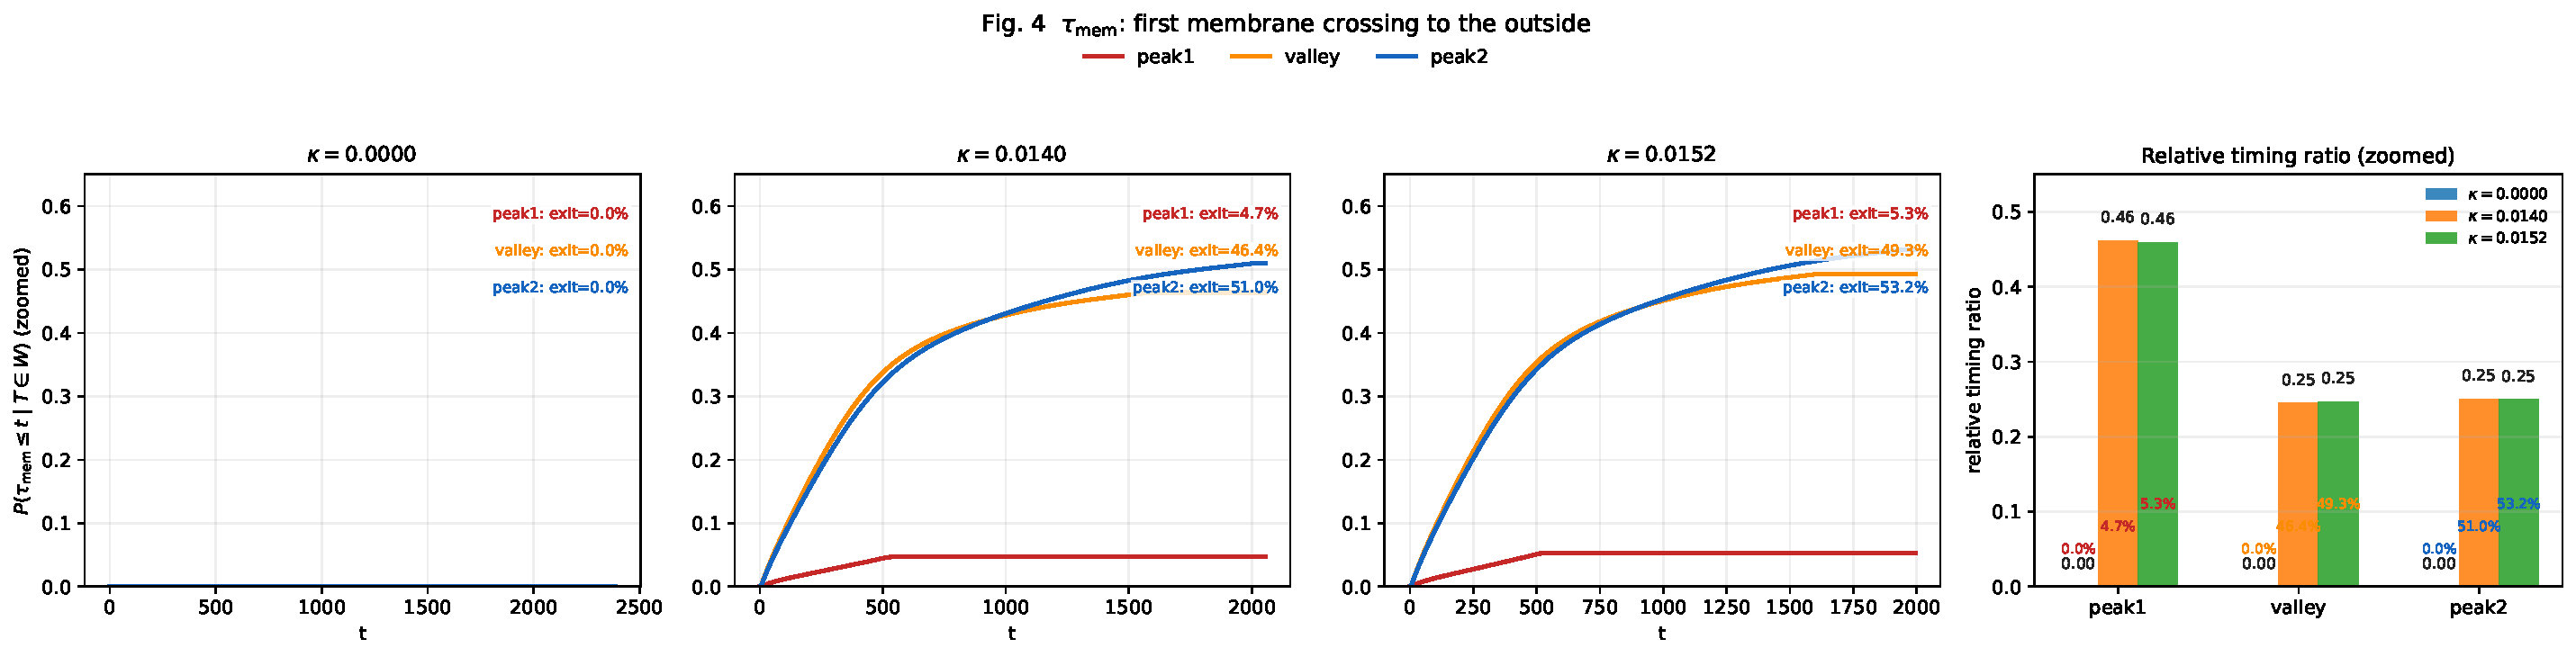
\includegraphics[width=0.98\linewidth]{../artifacts/figures/fig4_tau_mem_timing.pdf}
  \caption{Window-conditioned CDFs and relative timing ratios for \(\tau_{\mathrm{mem}}\). The \(\kappa=0\) panel is the strict zero control; the other two panels show takeover onset at \(\kappa=0.0140\) and the last phase-1 case at \(\kappa=0.0152\). To make the membrane-exit growth inside the critical band readable, both the CDF panels and the ratio panel use zoomed vertical scales.}
  \label{fig:tau-mem}
\end{figure}

Figure~\ref{fig:tau-mem} separates corridor leaving from genuine membrane crossing.

First, all three windows give exactly zero membrane-exit probability at \(\kappa=0\), which is the required sanity check.

Second, focusing directly on the two mechanism thresholds \(\kappa=0.0140\) and \(\kappa=0.0152\), we find
\[
P(\tau_{\mathrm{mem}}<T\mid T\in\texttt{peak1})\approx 4.68\%\ \text{to}\ 5.31\%,
\]
\[
P(\tau_{\mathrm{mem}}<T\mid T\in\texttt{valley})\approx 46.37\%\ \text{to}\ 49.33\%.
\]
\[
P(\tau_{\mathrm{mem}}<T\mid T\in\texttt{peak2})\approx 51.02\%\ \text{to}\ 53.16\%.
\]
The later windows are therefore exactly where membrane crossing becomes decisive: the representative critical-band cases sit right at the point where membrane-assisted trajectories become the majority inside the late branch.

Third, the timing ratio
\[
\frac{E[\tau_{\mathrm{mem}}\mid \tau_{\mathrm{mem}}<T,\ T\in W]}{E[T\mid T\in W]}
\]
is still only about \(0.25\) in both the valley window and the late peak. So even near takeover, whenever membrane crossings do matter, they still tend to occur in the earlier part of the corresponding late trajectories.

\section{Early / Late / No-Exit Decomposition}
The report also builds a coarser window-level split. For each window \(W\), we first compute \(E[T\mid T\in W]\) and then declare an event to be `early` whenever
\[
\tau \le 0.5\,E[T\mid T\in W].
\]
The remaining event mass is `late`, and paths with no such event contribute to `no exit`.

\begin{figure}[!htbp]
  \centering
  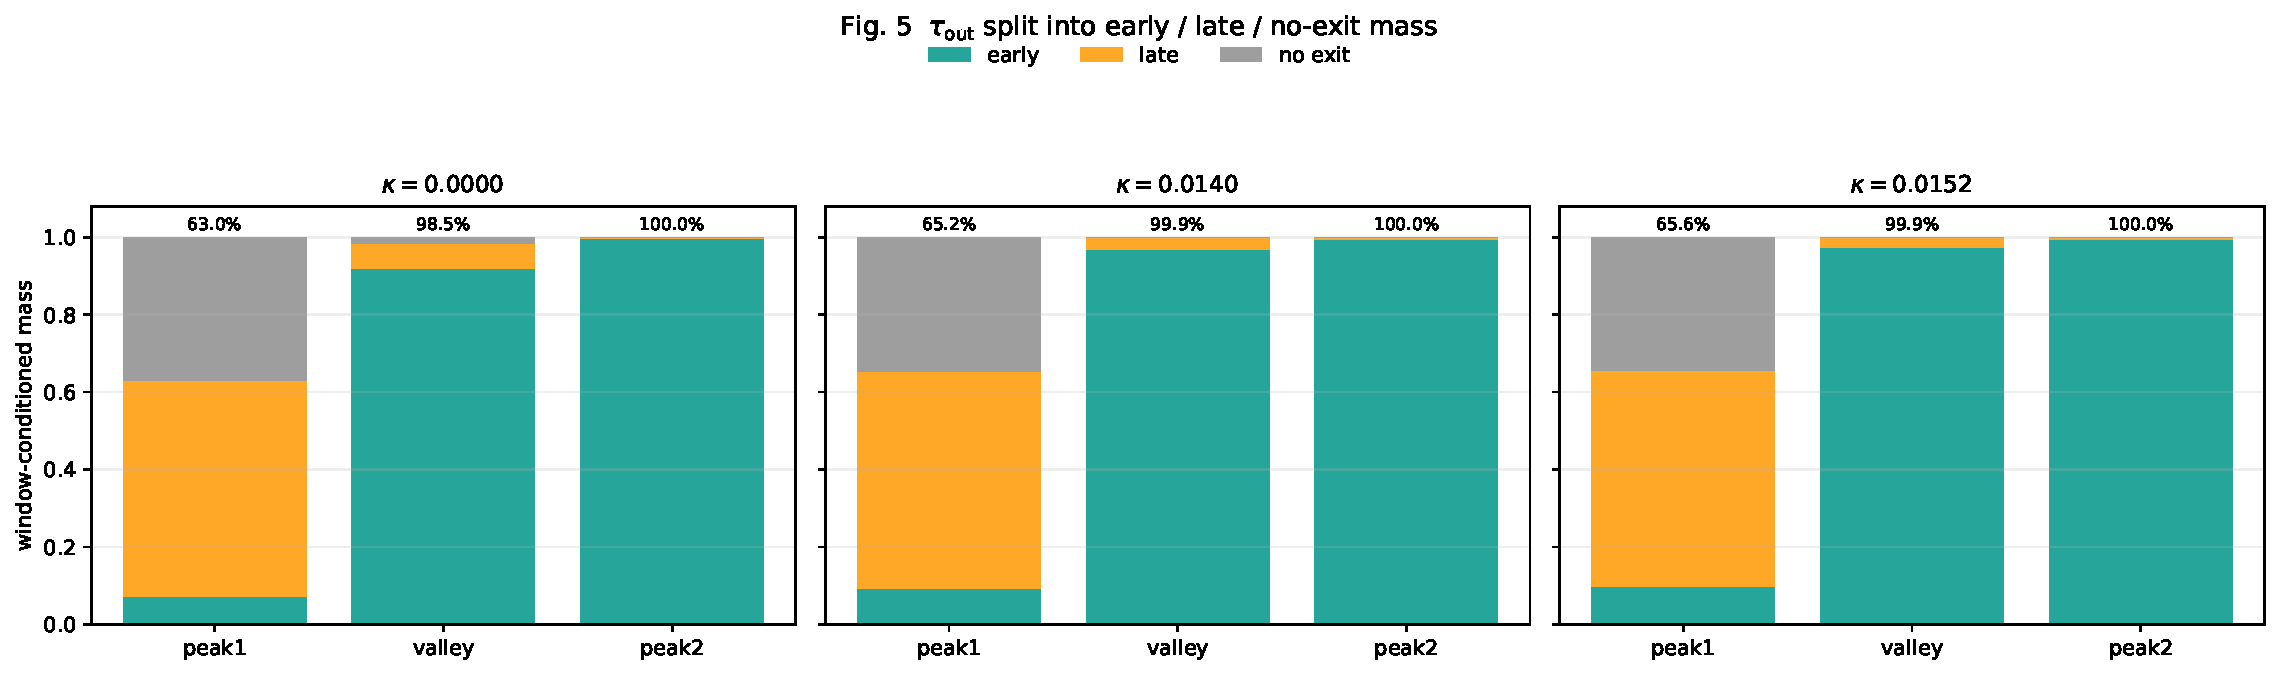
\includegraphics[width=0.98\linewidth]{../artifacts/figures/fig5_tau_out_split.pdf}
  \caption{Early / late / no-exit decomposition for \(\tau_{\mathrm{out}}\), shown for \(\kappa=0\), takeover onset \(\kappa=0.0140\), and the last phase-1 point \(\kappa=0.0152\). The number above each bar is the total exit mass.}
  \label{fig:tau-out-split}
\end{figure}

\begin{figure}[!htbp]
  \centering
  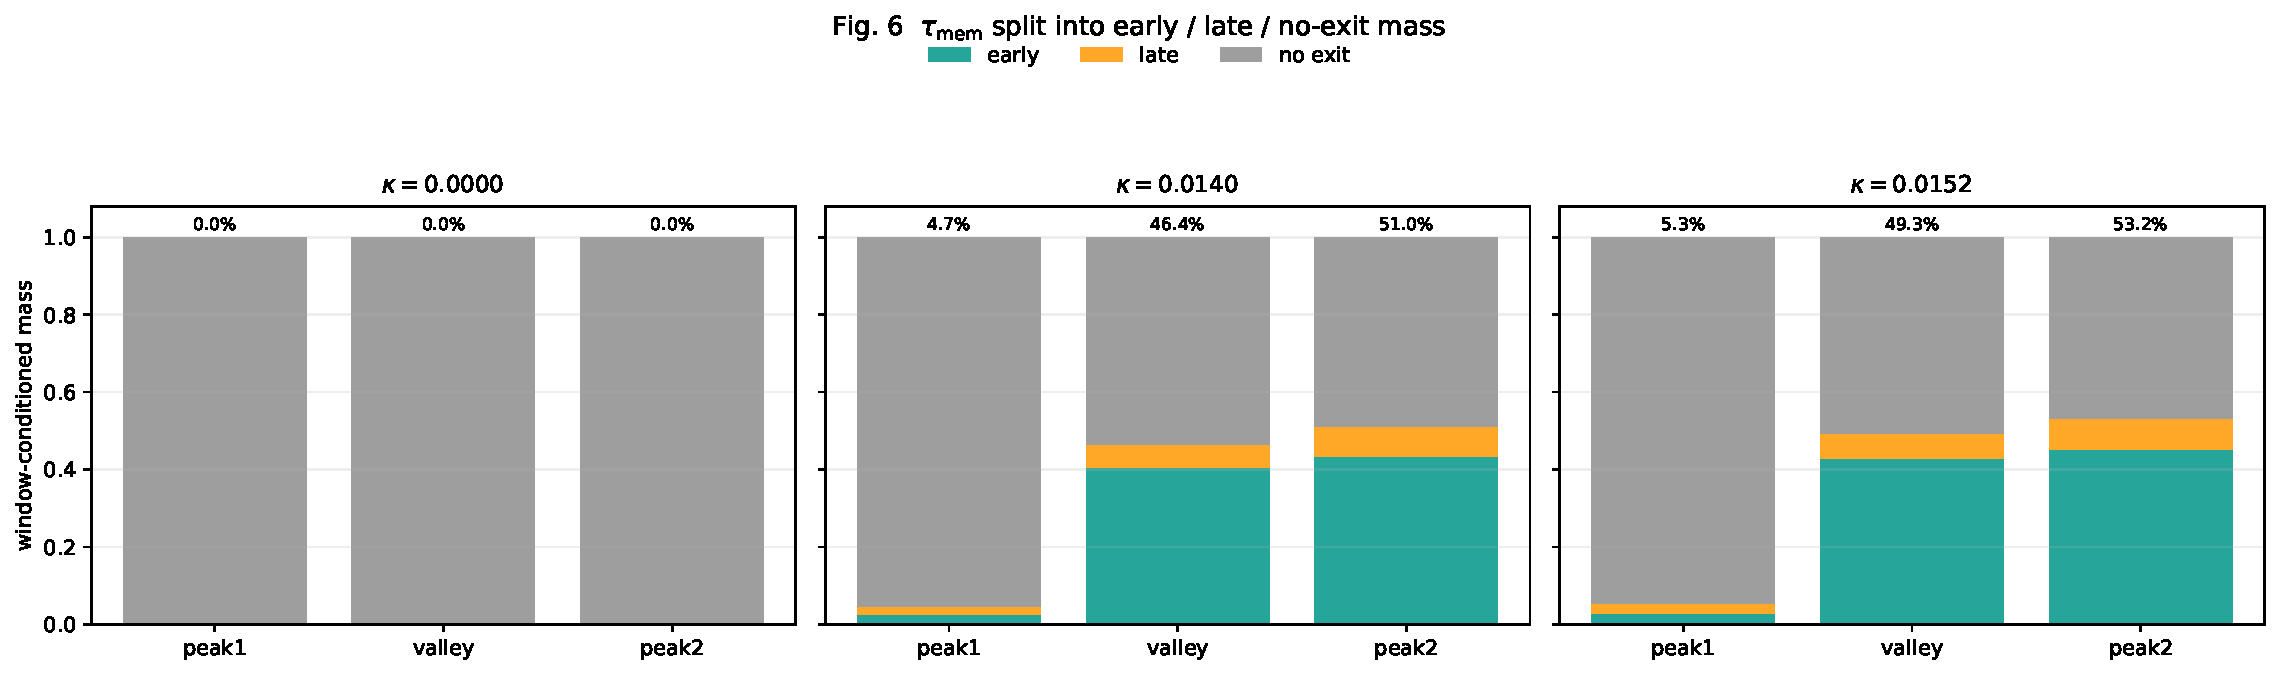
\includegraphics[width=0.98\linewidth]{../artifacts/figures/fig6_tau_mem_split.pdf}
  \caption{Early / late / no-exit decomposition for \(\tau_{\mathrm{mem}}\), using the same three mechanism representatives. At \(\kappa=0\), all three bars collapse to pure `no exit`, as they should.}
  \label{fig:tau-mem-split}
\end{figure}

Figures~\ref{fig:tau-out-split} and~\ref{fig:tau-mem-split} give the cleanest mechanism comparison.

For \(\tau_{\mathrm{out}}\), the valley and late-peak windows are almost entirely early-exit trajectories. This means that the distinctive feature of the slow branch is not whether it leaves the corridor, but how long it spends wandering before coming back.

For \(\tau_{\mathrm{mem}}\), by takeover onset and at the last phase-1 point the late windows are no longer dominated by `no exit`; but among the paths that do cross a membrane, most of the mass is still early rather than late. A compact interpretation is:
\begin{quote}
Membrane crossings add a slow membrane-assisted subfamily to the later windows, and near takeover that subfamily becomes the majority. Even so, its first crossing typically still happens relatively early.
\end{quote}
Figure~\ref{fig:takeover} then adds the next step: if \(\kappa\) is pushed further, this membrane-assisted subfamily does eventually take over the late peak, but only right before the bimodality collapses.

\section{Representative Table}
\begin{table}[!htbp]
  \centering
  \footnotesize
  \begin{tabular}{llcccc}
\toprule
$\kappa$ & Observable & peak1 exit & valley exit & peak2 exit & peak2 ratio \\
\midrule
0.0000 & $\tau_{\mathrm{out}}$ & 63.0\% & 98.5\% & 100.0\% & 0.16 \\
0.0000 & $\tau_{\mathrm{mem}}$ & 0.0\% & 0.0\% & 0.0\% & 0.00 \\
0.0140 & $\tau_{\mathrm{out}}$ & 65.2\% & 99.9\% & 100.0\% & 0.12 \\
0.0140 & $\tau_{\mathrm{mem}}$ & 4.7\% & 46.4\% & 51.0\% & 0.25 \\
0.0152 & $\tau_{\mathrm{out}}$ & 65.6\% & 99.9\% & 100.0\% & 0.12 \\
0.0152 & $\tau_{\mathrm{mem}}$ & 5.3\% & 49.3\% & 53.2\% & 0.25 \\
\bottomrule
\end{tabular}

  \caption{Representative \(\kappa\) values, showing window-conditioned exit probabilities and the \texttt{peak2} timing ratio for both observables.}
  \label{tab:rep}
\end{table}

Table~\ref{tab:rep} is the shortest numerical summary of the report. If one only remembers one contrast, it should be this:
\begin{itemize}
  \item at \(\kappa=0\), all three \(\tau_{\mathrm{mem}}\) probabilities are zero, while \(\tau_{\mathrm{out}}\) is already \(98.5\%\) and \(100\%\) in the valley and late peak;
  \item at \(\kappa=0.006\), the late-peak membrane-exit probability is still only about \(27.9\%\), far smaller than the corresponding corridor-exit probability, which is effectively \(100\%\).
\end{itemize}
That contrast almost fully answers the mechanism question: the second peak is driven primarily by leaving the corridor and taking outside detours, not by membrane crossings themselves.

\section*{Summary}
Viewed across the full continuation from fully reflective to weakly permeable, the most robust mechanism picture is:
\begin{enumerate}
  \item the first peak is dominated by direct corridor transport;
  \item the second peak already exists at \(\kappa=0\), showing that the baseline slow branch comes from outside detours accessible through the left opening;
  \item symmetric membrane permeability adds a membrane-assisted late subfamily; by \(\kappa=0.006\) it is clearly visible, but it still remains secondary under the present parameters;
  \item if \(\kappa\) is pushed into the critical band, the membrane-assisted mass in \texttt{peak2} exceeds \(50\%\) around \(\kappa\approx 0.014\), but this takeover survives only until the immediate pre-collapse regime because by \(\kappa=0.0153\) the bimodality is already gone;
  \item therefore \(\tau_{\mathrm{out}}\) is the primary observable for understanding who contributes the second peak, while \(\tau_{\mathrm{mem}}\) is the right follow-up observable for quantifying what the membrane adds on top of that baseline.
\end{enumerate}

\end{document}
